\documentclass{article}

\usepackage[utf8]{inputenc}
\usepackage[0T1]{fontenc}
\usepackage[french]{babel}
\usepackage{natbib}
\usepackage{graphicx}
\usepackage{setspace}
\usepackage[a4paper,bindingoffset=0.2in,%
            left=1in,right=1in,top=1in,bottom=1in,%
            footskip=.25in]{geometry}
\onehalfspacing

\begin{document}
    \begin{center}
        \rule{1.05\textwidth}{2pt}\\
            \Huge Mémoire de projet de data mining\\
            \huge \textbf{Sujet : Analyse des relevés des notes des étudiants de l'ENSIAS}\\
        \rule{1.05\textwidth}{2pt}\\
    \end{center}
    \newpage
        \section{La compréhension métier}
            Cette première phase consiste à bien comprendre les éléments métiers et la problématique qu’on vise à résoudre. On va commencer par déterminer les objectifs stratégiques et opérationneles. Puis, on va évaluer la situation actuelle. Finallement, vient la traduction de l’objectif stratégique en concepts de Data mining.\\
            \subsection{Détermination des objectifs stratégiques et opérationnelles}
                Le problème qu’on rencontre dans le travail de groupe dans notre école l’ENSIAS c’est la non homogénéité des groupes. Le seul facteur de la formation de ces groupes c’est la relation entre les membres. Ainsi les outils techniques peuvent ne pas plaire tous les membres d’un groupe. D’où vient l’idée de notre projet, former des groupes homogènes des étudiants ayant les mêmes compétences pour qu’ils puissent travailler sur un projet qui exploite leurs compétences communes. Tous cela, en annalysant leurs résultats et chercher les élèves ayant des résultats similaires dans la même fillière.\\
            \subsection{Analyse de la situation actuelle}
                Actuellement, nous disposons de quelques relevés de notes de la deuxième année de quelques filières : la filière e-Management et Business Intelligence (eMBI), la filière Génie Logiciel (GL) et les notes de la première année. Tous ces relevés de notes sont de la promotion de l’année 2021. Nous devons encore collecter les relevés de notes d’autres filières : la filière Ingénierie e-Logistique (IeL), la filière Ingénierie des Systèmes Embarqués et Mobiles (ISEM) et et la filière Sécurité des Systèmes d'Information (SSI).\par
                Parmi les problèmes que nous avons rencontrés c’est la sensibilité des données. On ne peut pas diffuser telles données personnelles, donc on doit cacher les noms et les prénoms des étudiants pour protéger leurs confidentialités.\\
            \subsection{Détermination des objectifs du Data Mining}
                Puisque l’objectif stratégique est clairement défini, il convient maintenant de le traduire en concepts de Data Mining. On va opter à une technique descriptive car nous sommes en train de présenter une information cachée par le volume des données. Et plus spécifiquement on va travailler un problème de clustering qui sert à regrouper des données non étiquetées présentant des propriétés similaires. Dans notre cas les proprités sont les notes de chaque module.\\
                \subsubsection{Clustering}
                    Le Clustering ou le partionnement des données est une méthode de classification non supervisée rassemble un ensemble d’algorithmes d’apprentissage pour relever des sous-ensembles des données difficiles à identifier à l’œil nu.\par
                    Pour atteindre ce but, cette technique vise à maximiser l’inertie entre les sous-ensembles pour bien les différencier et minimiser celle au sein du même ensemble pour qu’il soit plus homogène. Il existe plusieurs méthodes de clustering : méthodes hiérarchiques, méthodes de partitionnement et méthode mixtes.\\
                \subsubsection{K-means}
                    Nous avons  choisis travailler avec l’algorithme de K-means c’est un algorithme de partionnement qui permet de regrouper les observation de notre data set en K clusters distincts. L’algorithme de K-means est comme suit :\\
                    \begin{figure}[h!]
                        \centering
                        \fbox{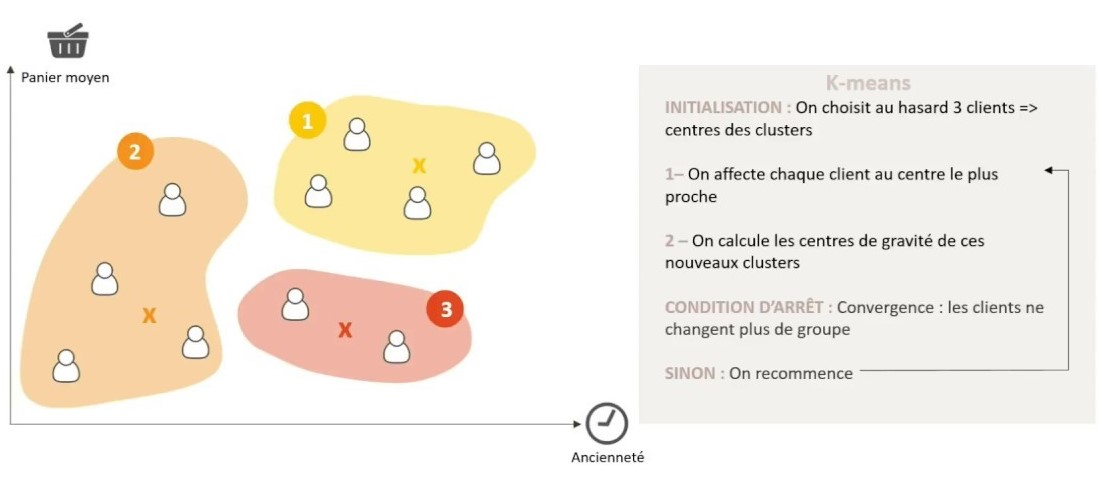
\includegraphics[scale=0.5]{kmeans}}
                        \caption{Principe algorithmique de K-means}
                        \label{fig:Kmeans}
                    \end{figure}
    \newpage
        \section{La compréhension des données}
            La phase de compréhension des données de CRISP-DM implique l’étude des données disponibles pour le Data mining. On doit tout d’abord collecter les données puis faire la description de ces données. La troisième étape est l’exploration des données et comme étape finale vérifier la qualité des données collectées.\\
            \subsection{Collecte des données}
                Nous avons pu collecter les notes de toute la promotion 2020 dans toutes les fillière auprès des élèves de cette promotion. Les notes de la première année qui est une année commune à toutes les filières. Puis les notes des élèves de chaque filière : eMBI, GL, IeL, SSI, et ISEM en deuxième année.\par
                \begin{figure}[h!]
                    \centering
                    \fbox{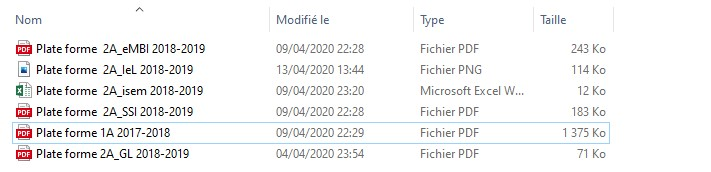
\includegraphics[scale=0.8]{data}}
                    \caption{Les données collectées}
                    \label{fig:data}
                \end{figure} 
                Nos fichiers sont de différents formats : des fichiers pdf, un fichier png et un fichier Microsoft Excel.\\
            \subsection{Description des données}
                Chaque fichier contient le nom et le prénom de l’étudiant, le moyen dans chaque semestre et chaque module ainsi la décision finale.\\
                \begin{figure}[h!]
                    \centering
                    \fbox{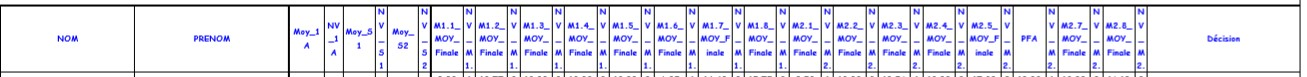
\includegraphics[scale=0.45]{columns}}
                    \caption{Les composants de chaque fichier}
                    \label{fig:columns}
                \end{figure} 
                \begin{flushright}
                    \begin{tabular}{| c | c | c | c | }
                        \hline
                        Code & Signification & Type & Longueur \\ \hline
                        NOM & Le nom de l’étudiant & Texte & 32 \\  \hline
                        PRENOM & Le prénom de l’étudiant & Texte & 32 \\ \hline
                        Moy_1A & Le moyen de la première année & Numérique & 5 \\  \hline
                        Moy_S1 & Le moyen de la première semestre de la première année & Numérique & 5 \\  \hline
                        Moy_S2 & Le moyen de la deuxième semestre de la première année & Numérique & 5 \\  \hline
                        NV_1A & Le nombre des modules non validé dans la première année & Numérique & 2 \\  \hline
                        NV_S1 & Le nombre des modules non validé dans & Numérique & 1 \\ 
                        & la première semestre de la première année & & \\ \hline
                        NV_S2 & Le nombre des modules non validé dans & Numérique & 1 \\
                        & la deuxième semestre de la première année & & \\ \hline
                        Mx.y_MOY_Finale & Le moyen du yème module dans la xème semestre & Numérique & 5 \\  \hline
                        NV_Mx.y & Le module y de la xème semestre est-il valide ?
•	0 : si le module est validé (Mx.y_MOY_Finale >=12)
•	1 : si le module n’est pas validé
 & Numérique & 5 \\  \hline
                        \hline
                    \end{tabular}
                \end{flushright}
\section{Conclusion}
``I always thought something was fundamentally wrong with the universe'' \citep{adams1995hitchhiker}

\bibliographystyle{plain}
\bibliography{references}
\end{document}
